\documentclass[conf]{new-aiaa}
\usepackage[utf8]{inputenc}

\usepackage{subcaption}
\usepackage{placeins}
\usepackage{cleveref}
\usepackage{graphicx}
\usepackage{amsmath}
\usepackage[version=4]{mhchem}
\usepackage[per-mode=symbol,separate-uncertainty = true,multi-part-units=single]{siunitx}
\usepackage{longtable,tabularx}
\setlength\LTleft{0pt} 
\usepackage{color}
\usepackage{epstopdf}
\usepackage{makecell}
\usepackage{url}
\usepackage{multirow}
\usepackage{float}
\usepackage[normalem]{ulem}

\usepackage{hyperref}

\sisetup{group-separator = {,}}

\graphicspath{{Figures/}}

\Crefname{equation}{Eq.}{Eqs.}
\Crefname{figure}{Fig.}{Figs.}

\DeclareSIUnit\inch{in}
\DeclareSIUnit\foot{ft}
\DeclareSIUnit\year{yr}
\DeclareSIUnit\knot{kts}
\DeclareSIUnit\poundforce{lbf}
\DeclareSIUnit\pixel{px}

\begin{document}

\begin{titlepage}

	\centering
	\vspace*{\fill}
	\rule{\textwidth}{0.4pt}
	\textsc{\huge Flight Test Report \\}
	\textsc{\huge Flight Test 04 (Aircraft Performance) \\}
	\bigskip
	\textsc{\large Date Submitted: May 11, 2020\\}
	\bigskip
	{\large Prepared by: \textsc{\huge Team Ramrod}\\}
	{(Shawn M. Herrington, Paul Klappa and Cody Smith)}	
	\rule{\textwidth}{0.4pt}
	
	\vspace*{\fill}	
	
	\begin{figure}[hbt!]
		\centering
		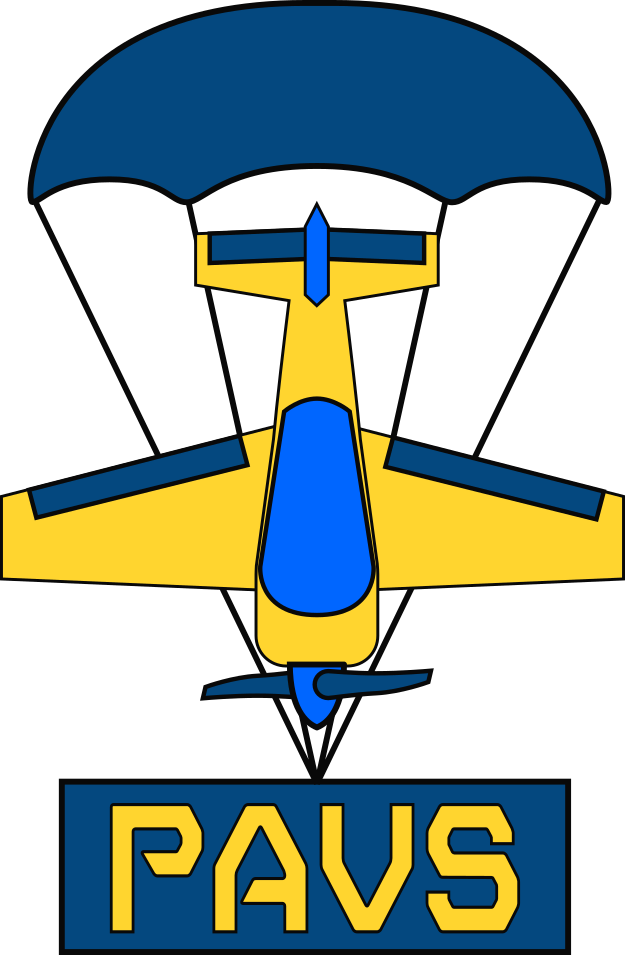
\includegraphics[height=1.75in]{PAVSLogo_BlackOutline.png}
		\label{PAVSLOGO}
	\end{figure}	
		
\end{titlepage}

\section{Introduction}

Assessing the flight performance characteristics of an aircraft is important when considering the aircraft capabilities. This test campaign focused on the assessment of the Piper Warrior II PA-28 and the Thorp T-18 – N249R series aircrafts while performing the level flight, climb, descent, takeoff, and landing maneuvers. Each maneuver has a characteristic airspeed that was recorded during the respective flight card maneuvers which will be discussed in more detail. 

\subsection{Test Objectives}

Level power required is determined during the level acceleration maneuver. During this maneuver, the flaps are set to~\SI{0}{\degree}~and throttle is steadily reduced until the flight speed achieves the stall speed. Once this state is achieved, the throttle is increased to full in order to allow the aircraft to stabilize at a maximum speed. The level power is found by taking aircraft measurements of fuel quantity and flow rate.

The climb rate is found from conducting the steady climb maneuver. During this maneuver, the aircraft trim is set to a desired airspeed with throttle set to full. The climb goes through~\SI{4000}{\foot} MSL or until~\SI{3}{\minute}. 

The descent rate is found by performing the steady descent maneuver. Throttle is set to idle during this maneuver as the descent goes through~\SI{2500}{\foot} MSL or for~\SI{3}{\minute}. This maneuver assumes the aircraft is close to level.

The takeoff distance is found during the short-field takeoff maneuver. The known aircraft starting point and the point of takeoff is the desired distance. The point where the aircraft takes off is the moment where the brakes are released and the aircraft achieves acceleration (point where nose wheel contact is lost with the ground). 

Landing distance was determined during the short-field landing maneuver. The distance is the displacement of the point of nose wheel contact with the ground and the complete stop position on the runway. The aircraft touchdown is within~\SI{100}{\foot}~of the runway numbers in order to achieve comparable landing repetitions.

\subsection{Team Ramrod}

Team Ramrod was established in 2019 with the goal of dethroning Tech N9ne as the most famous hip-hop act from Kansas City. Originally conceived as a foursome, the group was reduced to their current lineup after MC Tim Layman left the group due to creative differences. Following the success of their double platinum eponymous debut album, Team Ramrod shocked the world by walking away from their lucrative careers in the music industry in order to pursue advanced degrees in Mechanical Engineering.

\subsubsection{Shawn Herrington}

Shawn Herrington was born in Kansas City but he's a Florida man at heart. Shawn has rarely met a swear word he didn't immediately take a liking to. Shawn's number one skill is knowing the exact moment when someone has left the room so he can start talking about them behind their back. Often stirred into a furious rage over the most mundane things, Shawn can be made to put on an entertaining demonstration of overreaction just by asking him simple questions such as ``How are you doing today?'' or ``Did you get that email about the assignment?''.

\begin{figure}[hbt!]
	\centering
	
\includegraphics[height=1.5in]{ShawnExotic2.jpg}
	\label{PAVSLOGO}
	\caption{Discount Hulk Hogan}
\end{figure}

During flight tests, Shawn contributes as little as possible.  He earned the dubious distinction of being the only ``pilot'' (used loosely here) to successfully crash the notoriously milquetoast Cessna 172 in two out of three CG configurations. Shawn's hobbies include eating Cheetos Puffs\textsuperscript{\textregistered} with a fork (to avoid getting dusty orange fingers) and telling boring stories about his dog.  Annoyingly, Shawn has been known to refer to people, even people he's not related to as ``brother''.

\subsubsection{Paul Klappa}

Paul ``The Klapp'' Klappa is originally from great frozen tundra of the remote northern state of Minnesota. In addition to understanding the sport of hockey, Paul is distinguished by the way he pronounces ``bag'', ``rag'', etc. Despite his prolific professional wrestling career, Paul never let fame go to his head and even returns to Minnesota from time to time to participate in the regular ice fishing competitions held at any of of the states' famous \num{10000} lakes.

\begin{figure}[hbt!]
	\centering
	
\includegraphics[height=1.5in]{KlappIsCookin2.jpg}
	\label{PAVSLOGO}
	\caption{Can you smell what the Klapp is cookin'?!}
\end{figure}	

As the youngest and most charismatic member of \emph{Team Ramrod} Paul plays public relations manager for the team. Paul's main contributions to the team are making sure he is holding the correct brand of energy drink during press conferences to keep up that sweet sponsorship money. When he is not serving as test engineer, or repeatedly saying ``proceed'' awkwardly into the headset microphone Paul enjoys pumping some iron, hitting up the vending machine, and wearing sweatpants.

\subsubsection{Cody Smith}

Cody Smith hails from the greater metropolitan Kansas City area. Born and bred in the~\num{816} Cody represented his hood all over the world as crew chief for the world famous United States Air Force (USAF) B52 aerobatic demonstration team. Now living the calm civilian life, Cody scratches the thrill-seeker itch by hand-launching foam airplanes at great risk to life and limb. Ever courageous in the face of unspeakable danger, Cody answers questions like ''Dude, did you see how close that propeller was to your arm?'' with a simple shrug; just another routine day for this former USAF Airman.

\begin{figure}[hbt!]
	\centering
	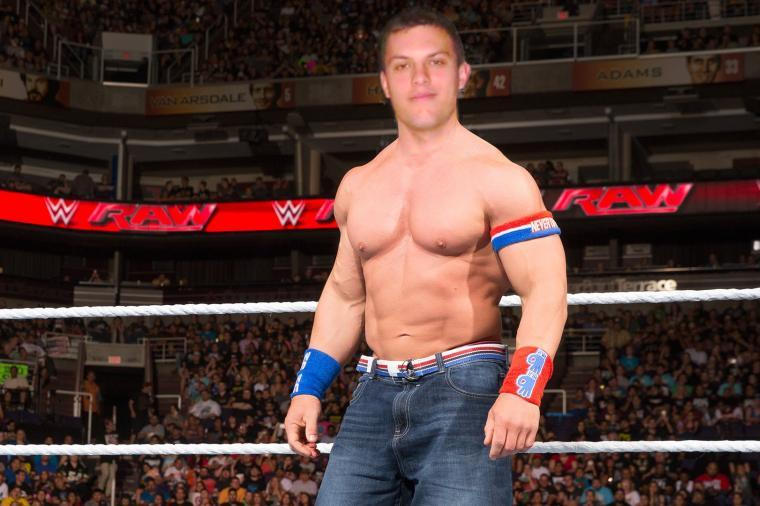
\includegraphics[height=1.5in]{CodyCena.jpg}
	\label{PAVSLOGO}
	\caption{Your time is up, my time is now!}
\end{figure}

Cody's role on \emph{Team Ramrod} is fashion consultant. Always dressed for the occasion, Cody is an expert on flight test engineering attire including cargo shorts and baseball caps. Due to his extensive experience working on real airplanes, Cody is always designated as the crew chief even when no crew chief is needed. When he's not pleading the case against Billy Joel to  his younger brother Simeon, Cody spends his free time watching his wife do squats and searching for that missing bag of trail-mix.


\section{Background}

\subsection{Level Flight Performance versus Power Required}

There are four forces on aircraft during flight. These forces are lift, weight, thrust, and drag. Lift acts perpendicular to the velocity. Drag acts parallel and opposite to velocity. Weight acts downward in the inertial reference frame. Finally, the thrust acts longitudinally in the body reference frame. The level flight performance in steady conditions relies on lift which is characterized by the following equations:

\begin{equation} \label{eq1}
\ L = W - T\sin(\theta_T)
\end{equation}

\begin{equation} \label{eq2}
\ D = T\cos(\theta_T)
\end{equation}

L is indicative of lift force, W is the weight, T is the thrust, and~$\theta_T$~is the angle of thrust. The drag force is produced as a by-product of lift and velocity. Aircrafts sustain flight by generating thrust to oppose drag. In order for the aircraft to achieve level flight performance, the following equations must be true:

\begin{equation} \label{eq3}
\ D_p = 1/2 \rho v^2 C_{D_p}
\end{equation}

\begin{equation} \label{eq4}
\ D_i = \frac{L^2}{1/2 \rho v^2 s \pi AR e}
\end{equation}

$D_{p}$~is the parasitic drag due to speed whereas~$D_{i}$~is the induced drag due to lift. ~$AR$~is the aspect ratio,~$e$~is the Oswald efficiency factor, and~$C_{D}$~is the drag coefficient.~$D_{p}$~will vary with~$v^{2}$~which is important to remember since increasing velocity will increase by the square of the velocity.~$D_{i}$~will vary with~$\frac{1}{v^2}$~which means induced drag decreases with increasing velocity.

The power required equation is based on force multiplied by the velocity. However, the power equation can be expanded into the following forms. It is important to note that power needs to be multiplied by about eight in order to achieve a velocity twice as fast.~$s$~represents the referenced frontal area of the aircraft (this reference can change depending on the geometry of the aircraft). The following equations show the substitutions required to yield the required power,~\textit{P}, equation.

\begin{equation} \label{eq5}
\ P = Dv
\end{equation}

\begin{equation} \label{eq6}
\ P = 1/2 \rho v^2 C_{D_p} s v
\end{equation}

\begin{equation} \label{eq7}
\ P = C_D s (1/2 \rho v^3)
\end{equation}

\begin{equation} \label{eq8}
\ D_p = 1/2 \rho v^2 C_{D_p} s
\end{equation}

\begin{equation} \label{eq9}
\ P = f (v^3)
\end{equation}

\subsection{Excess Power and Climbing Flight}
The climb performance of the aircraft follows the rate of climb equation where $\gamma$ is indicative of the flight path and not the propeller:

\begin{equation} \label{eq10}
\ R.O.C. = \frac{dH}{dt} = v \sin(\gamma)
\end{equation}

Climbing flight relies on the force from the time rate of change of height. Thrust horsepower excess, $THP_{excess}$, is another variable that is dependent on the height time rate of change and aircraft weight, $W$. 

\begin{equation} \label{eq11}
\ THP_{excess} = W \frac{dH}{dt}
\end{equation}

There is a power required curve for flight at specific velocities and a power available curve. The power required by the system is typically under the available power curve, and the excess thrust is the difference between the two curves. However, there is a point (crossover point) where more power is required to climb at a higher velocity than what is currently available for an aircraft. Thus, knowing the best angle of climb is important. The best angle of climb occurs right before the peak of the rate of climb on the R.O.C. plot versus velocity. There is also a best angle where the aircraft is flown steeply as possible to avoid low altitude obstacles. Once the obstacles are cleared, the best rate of climb is used. 

\subsection{Gliding Flight}

\subsection{Takeoff and Landing Performance}

\section{Test Procedure}

\begin{itemize}
	\item Overview of processes and equipment
	\item Narrative of the test procedure and equipment
	\item Anomalies or issues encountered
	\item Flight card
	\begin{itemize}
		\item Narrative in the text
		\item Scan in the appendix
	\end{itemize}
\end{itemize}

\section{Test Results}

\begin{itemize}
	\item Show plots of takeoff performance
	\item Show plots of level flight acceleration
	\item Show plots of climbs and descents
	\item Show plots of landing performance
\end{itemize}

\section{Discussion}

\begin{itemize}
	\item Takeoff and landing performance
	\begin{itemize}
		\item Ground roll
		\item Over \SI{50}{\foot} obstacle
		\item Compare distances with published data
	\end{itemize}
	\item Power required for level flight
	\begin{itemize}
		\item Show power required vs. airspeed plot (individual points and regression, if appropriate)
		\item Identify minimum power required and corresponding airspeed
		\item Identify maximum range and corresponding airspeed
		\item Compare airspeed with published data
	\end{itemize}
	\item Climb performance
	\begin{itemize}
		\item Show climb rate vs. airspeed climb polar (individual points and regression, if appropriate)
		\item Identify maximum climb rate and corresponding airspeed
		\item Identify maximum climb angle and corresponding airspeed
		\item Compare airspeeds with published data
	\end{itemize}
	\item Gliding performance
	\begin{itemize}
		\item Show descent rate vs. airspeed glide polar (individual points and regression, if appropriate)
		\item Identify maximum sink rate and corresponding airspeed
		\item Identify best glide speed and corresponding airspeed
		\item Compare airspeeds with published data
	\end{itemize}
\end{itemize}

\section{Conclusions}

\begin{itemize}
	\item Summary of test objectives
	\item Summary of process
	\item Summary of findings
	\item Recommendations
\end{itemize}

Innocuous changes in another section.

\section{Appendix}

Dummy github changes.

\end{document}
